\begin{marginfigure}[1cm]
\margingraphics{figures/1_3_Act3.eps} 
\caption{Axes for plotting $y = P(t)$ in Activity~\ref{A:2.1.3}.} \label{fig:2.1.Act3}
\end{marginfigure}

\begin{activity}  \label{A:2.1.3}
A rapidly growing city in Arizona has its population $P$ at time $t$, where $t$ is the number of decades after the year $2010$, modeled by the formula $P(t) = 25000 e^{t/5}$.  Use this function to respond to the following questions.
\ba
	\item Sketch an accurate graph of $P$ for $t = 0$ to $t = 5$ on the axes provided in Figure~\ref{fig:2.1.Act3}.  Label the scale on the axes carefully.
	
	\item Compute the average rate of change of $P$ between $2030$ and $2050$.  Include units on your answer and write one sentence to explain the meaning (in everyday language) of the value you found.
	\item Use the limit definition to write an expression for the instantaneous rate of change of $P$ with respect to time, $t$, at the instant $a = 2$.  Explain why this limit is difficult to evaluate exactly.  
	\item Estimate the limit in (c) for the instantaneous rate of change of $P$ at the instant $a = 2$ by using several small $h$ values.  Once you have determined an accurate estimate of $P'(2)$, include units on your answer, and write one sentence (using everyday language) to explain the meaning of the value you found.
	\item On your graph above, sketch two lines:  one whose slope represents the average rate of change of $P$ on $[2,4]$, the other whose slope represents the instantaneous rate of change of $P$ at the instant $a=2$.
	\item In a carefully-worded sentence, describe the behavior of $P'(a)$ as $a$ increases in value.  What does this reflect about the behavior of the given function $P$?
\ea
\end{activity}
\begin{smallhint}
\ba
	\item $P(t)$ is the standard exponential function, scaled by $25000$.
	\item Use the formula for the average rate of change of a function.
	\item Because of the exponential nature of $P(t)$, we're not able to simplify $\frac{P(2+h)-P(2)}{h}$ in a way that removes $h$ from the denominator.  
	\item Try using $h = 0.001, 0.0001, 0.00001$ and $h = -0.001, -0.0001, -0.00001$.  Be careful not to round or use computing precision that is too limited.  
	\item For the first line, think about the points $(2,P(2))$ and $(4,P(4))$.
	\item Visualize the slope of the tangent line and how it changes as a point moves along the curve.
\ea
\end{smallhint}
\begin{bighint}
\ba
	\item $P(t)$ is the standard exponential function, scaled by $25000$.
	\item Remember that $AV_{[2,4]} = \frac{P(4)-P(2)}{4-2}$, and that the units on $P$ are people, while $t$ is the number of decades after 2010. 
	\item Note that
	$$P'(2) = \lim_{h \to 0} \frac{P(2+h)-P(2)}{h} = \lim_{h \to 0} \frac{25000 e^{2+h}-25000e^2}{h}.$$  
	\item Try using $h = 0.001, 0.0001, 0.00001$ and $h = -0.001, -0.0001, -0.00001$.  Be careful not to round or use computing precision that is too limited.  Think about how using the two values of $h$ nearest 0 together could give you the most accurate result.
	\item For the first line, think about the points $(2,P(2))$ and $(4,P(4))$.  For the second, try the line through $(2,P(2))$ with slope $P'(2)$.
	\item Visualize the slope of the tangent line and how it changes as a point moves along the curve.  Does the slope of the tangent line increase, decrease, or stay the same as the point of tangency moves along the curve from right to left?
\ea
\end{bighint}
\begin{activitySolution}
\ba
	\item 	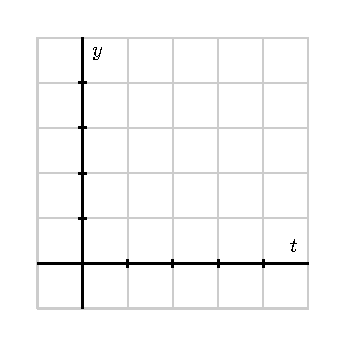
\includegraphics{figures/1_3_Act3.eps}
	\item $AV_{[2,4]} = \frac{P(4)-P(2)}{4-2} = \frac{25000e^{4/5} - 25000e^{2/5}}{2} \approx 9171$ people per decade is expected to be the average rate of change of the city's population over the two decades from 2030 to 2050.
	\item Note that
	\begin{eqnarray*} P'(2) & = & \lim_{h \to 0} \frac{P(2+h)-P(2)}{h} = \lim_{h \to 0} \frac{25000 e^{(2+h)/5}-25000e^{2/5}}{h} \\
	                                 & = &  \lim_{h \to 0} \frac{25000 e^{2/5} e^{h/5} -25000e^{2/5}}{h} =  \lim_{h \to 0} 25000e^{2/5}\left( \frac{e^{h/5} - 1}{h}\right)	\end{eqnarray*}
Because there is no way to remove a factor of $h$ from the numerator, we cannot eliminate the $h$ that is making the denominator go to zero, so it appears we need to be content estimating the limit with small values of $h$.
	\item Using $h = 0.00001$, we find $\frac{P(2+0.00001)-P(2)}{0.00001} \approx 7457$; using $h = -0.00001$, we find $\frac{P(2-0.00001)-P(2)}{-0.00001} \approx 7460$.  Averaging these two results, we find that
	$$P'(2) =  \lim_{h \to 0} \frac{P(2+h)-P(2)}{h} \approx 7458.5$$
	which is measured in people per decade.
	\item See the graph provided in (a) above.  The magenta line has slope equal to the average rate of change of $P$ on $[2,4]$, while the green line is the tangent line at $(2,P(2))$ with slope $P'(2)$.
	\item If we consider the point where $t = a$ and let $a$ start at 0 and then increase, it appears that the tangent line's slope at the point $(a,P(a))$ will increase as $a$ increases.
\ea
\end{activitySolution}
\aftera